\documentclass{beamer}
% Class options include: notes, handout, trans
%                        

\usepackage[french]{babel}
\usepackage[utf8]{inputenc}
\usepackage{calc}
\usepackage{tikz}
\usepackage{verbatim}

% Theme for beamer presentation.
\usepackage{beamerthemesplit} 
% Other themes include: beamerthemebars, beamerthemelined,beamerthemetree, beamerthemeplain

\usefonttheme{professionalfonts}

\title[Création d'un interface graphique pour Tikz]{Création d'un interface graphique pour Tikz}
\subtitle{PSTL encadré par Fréderic Pechanski}    % Enter your title between curly braces
%\author[L. Numbers]{Lucas Numbers}                 % Enter your name between curly braces
\author[]{Ancelin Maxime\\Diakhate Aminata}                 % Enter your name between curly braces
\institute[UPMC]{M1 Informatique spécialité STL\\UPMC}      % Enter your institute name between curly braces
\date{8 juin 2012}      % Enter the date or \today between curly braces

\usepackage{graphicx}

\begin{document}

\newenvironment{violetpar}{\color{violet}}{}
\newenvironment{bluepar}{\par\color{blue}}{\par}
\newenvironment{yellowpar}{\par\color{orange}}{\par}




%\renewcommand{\labelitemi}{$\bullet$}

%%%%%%%%%%%%%%%%%%%%%%%%===Slide 1 - Titre
\begin{frame}
  \titlepage
\ \ \ \begin{tikzpicture}[node distance=50pt]
\node[draw,circle,black,fill=blue!50,line width=3] (first_node) {Tikz};
\node[below of = first_node, node distance = 10] (first_node_y20) {};
\node[draw,circle,right of = first_node_y20, node distance = 21,fill=green!50,line width=2] (first_node_y20_x21) {g};
\node[below of = first_node, node distance = 40] (first_node_y) {};

\end{tikzpicture}
\   \ \ \ \ \ \ \ \ \ \ \ \ \ \ \ \ \ \ \ \ \ \ \ \ \ \ \ \ \ \ \

\includegraphics[width=5cm, height=3cm]{img/LogoUPMC.jpg} 
\end{frame}

%%%%%%%%%%%%%%%%%%%%%%%%===Slide 2 - Plan
\begin{frame}
\frametitle{Plan} 

\begin{itemize}

\item Objectifs du PSTL

\item Réalisation du projet

\item Résultats

\item L'avenir de TikzG


\end{itemize}
\end{frame}

%%%%%%%%%%%%%%%%%%%%%%%%===Slide 3 - OBJECTIFS DU PSTL
\begin{frame}
\frametitle{Objectifs du PSTL} 


\begin{itemize}

\item Création d'une interface graphique pour
faciliter\\ l'utilisation de Tikz.

\item Sous-ensemble de Tikz traité : nœuds,
arêtes.

\end{itemize}
\end{frame}

%%%%%%%%%%%%%%%%%%%%%%%%===Slide 4 - Réalisation du projet
\begin{frame}
\frametitle{Réalisation du projet} 


\begin{itemize}

\item Transformation du code Tikz en image

\item Création de l'interface graphique

\item Représentation mémoire des objets Tikz

\item Intéraction avec le graphe

\end{itemize}

\end{frame}

%%%%%%%%%%%%%%%%%%%%%%%%===Slide 5 - Transformation code Tikz
\begin{frame}
\frametitle{Transformation d'un code Tikz en image}
\centering
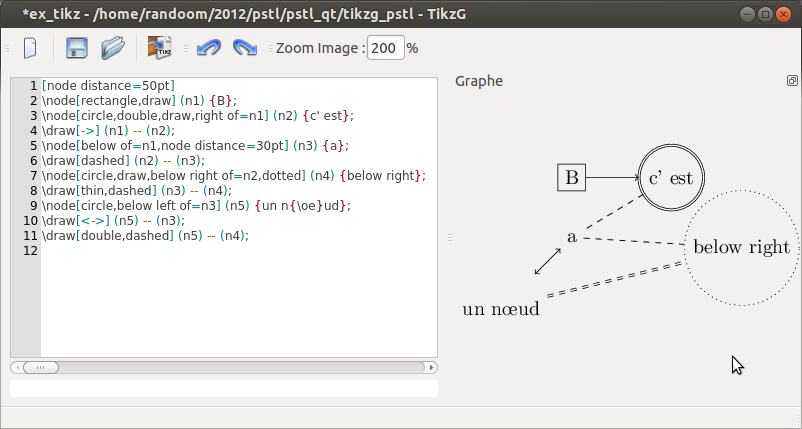
\includegraphics[width=10cm, height=6cm]{img/r_1.png}
\end{frame}

%%%%%%%%%%%%%%%%%%%%%%%%===Slide 6 - Transformation code Tikz
\begin{frame}
\frametitle{Transformation d'un code Tikz en image}
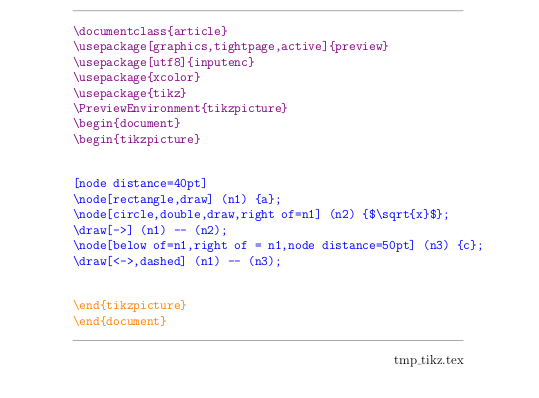
\includegraphics[width=10cm, height=4cm]{img/c1.png} \\
\begin{center}
$\overset{pdflatex\ -halt-on-error\ tmp\_tikz.tex\ >\ /dev/null }{\downarrow}$

\includegraphics[width=5cm, height=0.5cm]{img/re1.png} \\
\hspace{11mm}
{\normalsize $\downarrow$ \textit{convert}}\\
%$\overset{convert}{\downarrow}$ \\

\includegraphics[width=5cm, height=0.5cm]{img/re2.png} \\
\end{center}

\end{frame}

%%%%%%%%%%%%%%%%%%%%%%%%===Slide 7 - Objets Tikz
\begin{frame}

\frametitle{Représentation mémoire des objets Tikz}

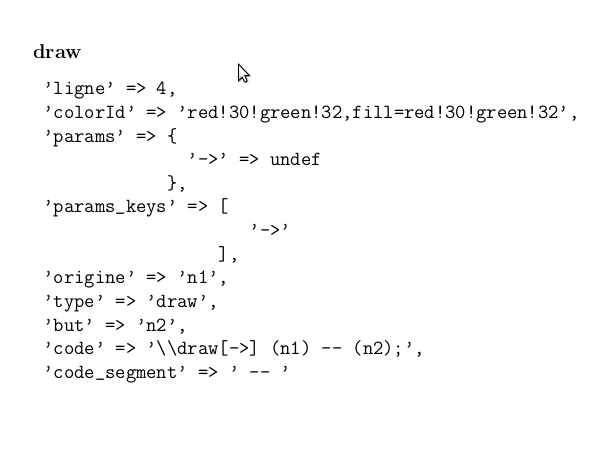
\includegraphics[width=5cm, height=5cm]{img/n3.png}
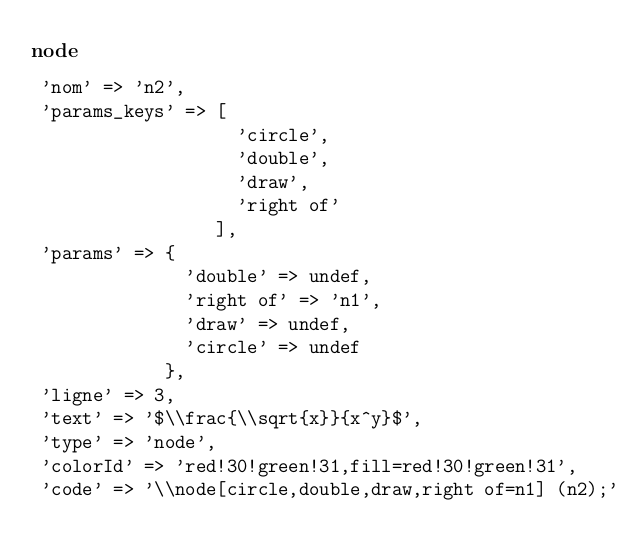
\includegraphics[width=7cm, height=5cm]{img/n2.png}\\
\centering
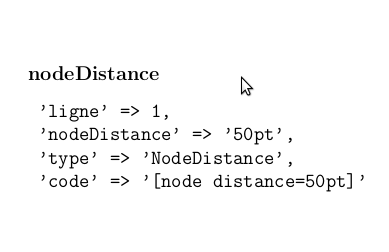
\includegraphics[width=5cm, height=3cm]{img/n1.png}
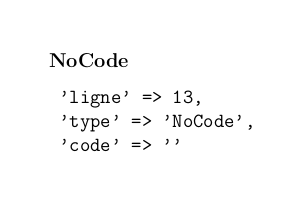
\includegraphics[width=5cm, height=3cm]{img/n4.png}
\end{frame}


%%%%%%%%%%%%%%%%%%%%%%%%===Slide 8 - Détection d'un objet Tikz
\begin{frame}
\frametitle{Détection d'un objet Tikz} 


\begin{itemize}

\item Détection basée sur une image auxiliaire

\end{itemize}

\vspace{5mm}
\begin{center}
\begin{tabular}{ccc}
\begin{tikzpicture}
[node distance=40pt]
\node[rectangle,draw] (n1) {a};
\node[circle,double,draw,right of=n1] (n2) {$\sqrt{x}$};
\draw[->] (n1) -- (n2);
\node[below of=n1,right of = n1,node distance=50pt] (n3) {c};
\draw[<->,dashed] (n1) -- (n3);
\end{tikzpicture} &
$\rightarrow$ &
\begin{tikzpicture}[node distance=40pt]
\node[rectangle,draw,red!30!green!30,fill=red!30!green!30] (n1) {a};
\node[circle,double,draw,right of=n1,red!30!green!31,fill=red!30!green!31] (n2) {$\sqrt{x}$};
\draw[line width=5pt,red!30!green!32,fill=red!30!green!32] (n1) -- (n2);
\node[below of=n1,right of = n1,node distance=50pt,red!30!green!33,fill=red!30!green!33] (n3) {c};
\draw[line width=5pt,red!30!green!34,fill=red!30!green!34] (n1) -- (n3);
\end{tikzpicture}
\\ 
tmp\_tikz.png &  & tmp\_tikz\_IDC.png \\ 
\end{tabular} 
\end{center}
\end{frame}


%%%%%%%%%%%%%%%%%%%%%%%%===Slide 9 - Détection ... - ajout IdColor
\begin{frame}[containsverbatim]
\frametitle{Détection d'un objet Tikz} 
\framesubtitle{Création image auxiliaire}
%\begin{itemize}
\begin{small}
\begin{verbatim}
[node distance=40pt]
\node[rectangle,draw] (n1) {a};
\node[circle,double,draw,right of=n1] (n2) {$\sqrt{x}$};
\draw[->] (n1) -- (n2);
\node[below of=n1,right of = n1,node distance=50pt] (n3) {c};
\end{verbatim}
\begin{flushright}
{\small \textit{code Tikz initial}}
\end{flushright}
\begin{center}
{\normalsize $\downarrow$ \textit{ajout des ColorID}}\\
\end{center}
\verb?[node distance=40pt]?\\
\verb?\node[rectangle,draw?\textcolor{red}{\textbf{,red!30!green!30,fill=red!30!green!30}}\verb?] (n1) {a};?\\
\verb?\node[circle,double,draw,right of=n1?\textcolor{red}{\textbf{,red!30!green!31,fill=red!30!green!31}}\verb?] (n2) {$\sqrt{x}$};?\\
\verb?\draw[?\textcolor{red}{\textbf{line width=5pt,red!30!green!32,fill=red!30!green!32}}] (n1) \verb?-- (n2);?
\verb?\node[below of=n1,right of = n1,node distance=50pt?\\\textcolor{red}{\textbf{,red!30!green!33,fill=red!30!green!33}}\verb?] (n3) {c};?\\
\begin{flushright}
{\small \textit{code Tikz avec ColorID}}
\end{flushright}
\end{small}
\end{frame}

%%%%%%%%%%%%%%%%%%%%%%%%===Slide 10 - Détection ... - Liste traduction IdColor -> RGB
\begin{frame}[containsverbatim]
\frametitle{Détection d'un objet Tikz} 
\framesubtitle{Traduction ColorID en RGB (et vice-versa)}
\begin{verbatim}
red!30!green!30 => 51657 59624 46003
red!30!green!31 => 51400 59367 45232
red!30!green!32 => 50886 59367 44461
red!30!green!33 => 50372 59110 43947
red!30!green!34 => 49858 58853 43176
red!30!green!35 => 49601 58596 42662
\end{verbatim}
\hrule
\begin{flushright}
\textit{6 premiéres lignes de \textbf{list\_IDC}}
\end{flushright}
\end{frame}

%%%%%%%%%%%%%%%%%%%%%%%%===Slide 11 - Détection ... - Liste traduction IdColor -> RGB
\begin{frame}
\frametitle{Détection d'un objet Tikz} 
\framesubtitle{Modification des propriétés de l'élément selectionné}
%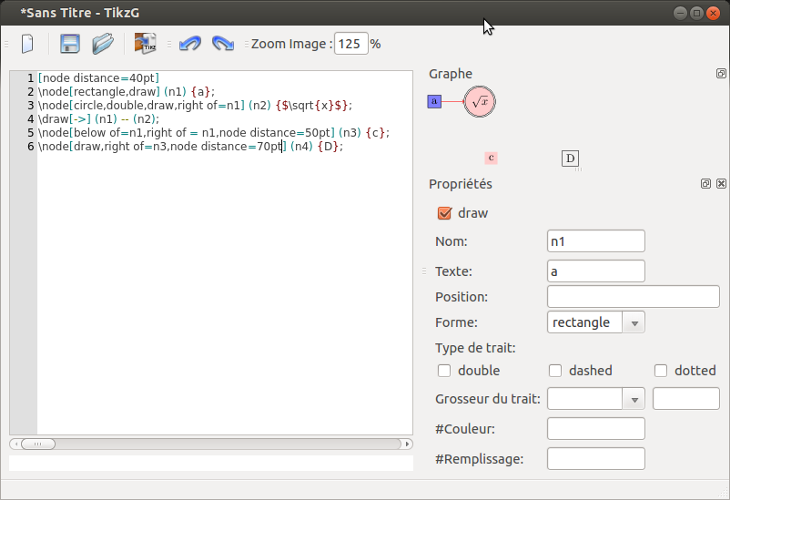
\includegraphics[width=12cm, height=10cm]{img_rel.png} 
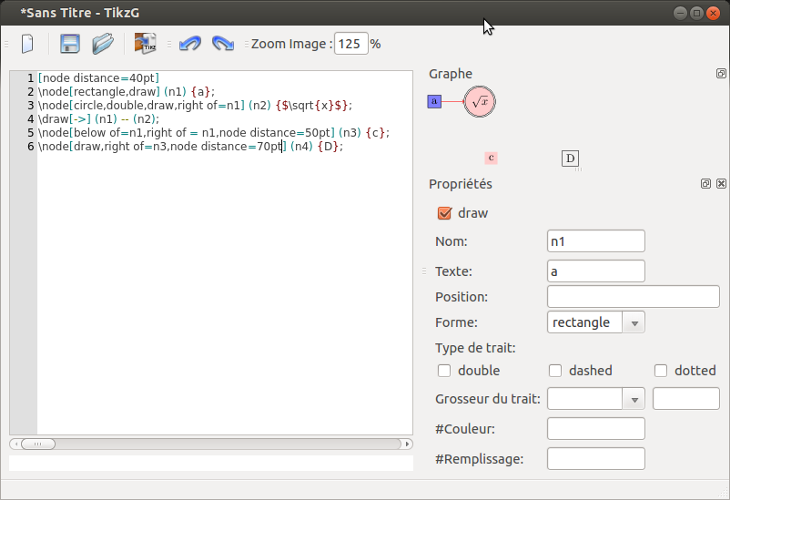
\includegraphics[scale=0.45]{img_rel.png} 
%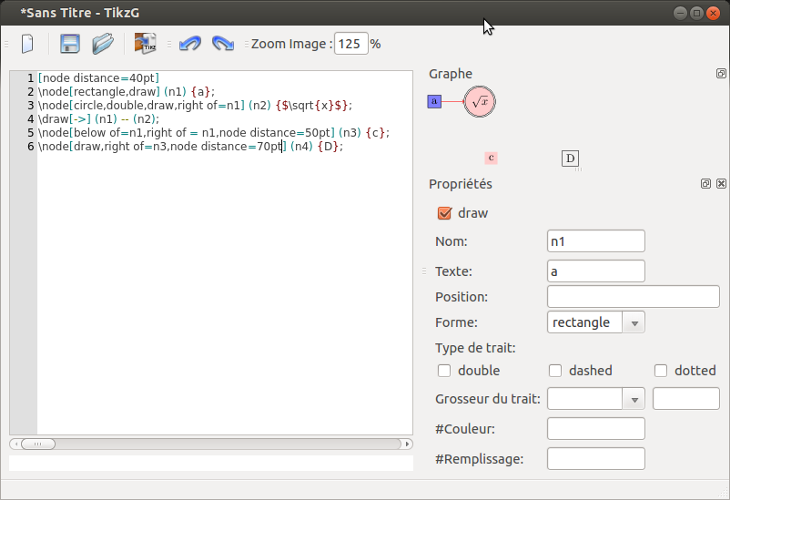
\includegraphics{img_rel.png} 
\end{frame}	

%%%%%%%%%%%%%%%%%%%%%%%%===Slide 12 - Création noeud aux coordonnées d'un clic
\begin{frame}
\frametitle{Création d'un n{\oe}ud aux coordonnées d'un clic} 
\framesubtitle{Principe}
Dans un graphe Tikz, tout n{\oe}ud peut être placé a une position précise en fonction du premier n{\oe}ud du graphe et d'un n{\oe}ud relatif a celui ci.
\\
\vspace{3mm}
\begin{tikzpicture}[node distance=120pt]
\node[rectangle,draw] (n1) {premier n{\oe}ud};
\node[draw,dashed,below of=n1] (n2) {n{\oe}ud auxiliaire invisible};
\draw[red] (n1.center) -- (n2.center) node[midway,right] {\textcolor{blue}{H (valeur pour "below of")}};
\node[draw,right of=n2,node distance=240pt] (n3) {n{\oe}ud final};
\draw[red] (n2.center) -- (n3.center) node[midway,below] {\textcolor{blue}{L (valeur pour "right of")}};


\end{tikzpicture}
\end{frame}

%%%%%%%%%%%%%%%%%%%%%%%%===Slide 13 - Création noeud aux coordonnées d'un clic - 1er étape
\begin{frame}
\frametitle{Création d'un n{\oe}ud aux coordonnées d'un clic} 
\framesubtitle{Premiére étape : calcul des coordonnées du centre du premier n{\oe}ud}
\begin{itemize}
\item Récupération des bornes du premier n{\oe}ud grâce au colorID
\end{itemize}
\begin{tikzpicture}[node distance=80pt]
\node[] (n1) {};
\node[below of=n1,node distance=30pt] (n2) {};
\node[right of=n1] (n3) {};
\node[right of=n2] (n4) {};
%\node[below right of=n1,node distance=20pt] (n5) {premier n{\oe}ud};
\draw(n1.center) -- (n2.center) node[midway,left] {\textcolor{blue}{x\_deb}};
\draw(n3.center) -- (n4.center) node[midway,right] {\textcolor{blue}{x\_fin}};
\draw(n1.center) -- (n3.center) node[midway,above] {\textcolor{blue}{y\_deb}};
\draw(n2.center) -- (n4.center) node[midway,below] {\textcolor{blue}{y\_fin}};
\node[below of = n1, node distance = 15] (n1_y15) {};
\node[rectangle,right of = n1_y15, node distance = 37] (n1_y15_x37) {premier n{\oe}ud};
\end{tikzpicture}

\begin{itemize}
\item Calcul des coordonnées (\textit{x},\textit{y}) du centre du premier n{\oe}ud
\end{itemize}
\begin{center}
\textit{x} = int((\textit{x\_fin} - \textit{x\_deb})/2 + \textit{x\_deb})

\textit{y} = int((\textit{y\_fin} - \textit{y\_deb})/2 + \textit{y\_deb})
\end{center}
\end{frame}

%%%%%%%%%%%%%%%%%%%%%%%%===Slide 14 - Création noeud aux coordonnées d'un clic - 2éme étape
\begin{frame}[containsverbatim]
\frametitle{Création d'un n{\oe}ud aux coordonnées d'un clic} 
\framesubtitle{Deuxiéme étape : création du n{\oe}ud intermédiaire et du n{\oe}ud final}
%Ces deux n{\oe}uds sont générés en fonction de l'écart en abscisse et en ordonnée entre la position du premier n{\oe}ud et celle du clic.
\begin{verbatim}
\node[draw] (n) {premier};
\node[below of = n, node distance = 41] (n_y41) {};
\node[draw,rectangle,right of = n_y41, node distance = 47]
 (n_y41_x47) {new};
\end{verbatim}
 
\begin{center}
{\normalsize \textcolor{blue}{$\downarrow$}}\\
\vspace{3mm}
\begin{tikzpicture}\node[draw] (n) {premier};
\node[below of = n, node distance = 41] (n_y41) {};
\node[draw,rectangle,right of = n_y41, node distance = 47] (n_y41_x47) {new};
\end{tikzpicture}


\end{center}

\end{frame}

%%%%%%%%%%%%%%%%%%%%%%%%===Slide 14 - Création noeud aux coordonnées d'un clic - 2éme étape
\begin{frame}
\frametitle{Création d'un n{\oe}ud aux coordonnées d'un clic} 
%\includegraphics[scale=0.45]{r_6.png} 
\includegraphics[scale=0.35]{img/r_6.png} 
\end{frame}

\end{document}

